\ This sections provides the simulated ETA results including the propagation of systematic nuclear data uncertainty. 
The neutron flux timing profile does not include the $\sigma_{sys}$ as the source mapping removed the time history data from the initial transport problem. 
First, the Monte Carlo simulation results pertaining to the neutron flux environment and foil pack activations are provided. 
The Monte Carlo results determined the effect of nuclear data covariance on the radiation transport simulation. 
Covariance analysis was only performed on ETA, not the objective TN+PFNS. 
As such, the final results are indicated by the MCNP-derived mean value with the bootstrapped uncertainty from the Sampler trials performed.
Next, the results of the neutron flux unfolding are shown which indicate the level of confidence of the foil pack to unfold the neutron flux for the ETA experiment. 
Finally, the fission product distribution and individual isotope production are provided. 

\section{ETA Monte Carlo Simulation Results}
\subsection{ETA Performance - Neutron Fluence Environment Comparison to TN+PFNS}

\ The main objective of ETA is to spectrally shape the DT source neutrons to the TN+PFNS.
Therefore, the spectrum achieved is a key metric for determining the performance of ETA.  
Figure \ref{fig:flux11} displays the nominal neutron fluence on the HEU foil as a function of energy with $\sigma_{stat}$ for the continuous energy neutron transport calculations.  
 
\begin{figure}[!htbp]
	\centering
	\vfill
	\subfigure[Logarithmic energy scale]{\includegraphics[width=13cm]{Figures/Chapter4/NeutronFlux/CE_Fluence_leth_c.png}}
	\vfill
	\subfigure[Linear energy scale]{\includegraphics[width=13cm]{Figures/Chapter4/NeutronFlux/CE_Fluence_leth_c_lin.png}}
	\vfill
	\caption{Neutron fluence per unit lethargy for SCALE MAVRIC, MCNP and objective TN+PFNS spectra. Only $\sigma_{stat}$ is captured for these results.}
	\label{fig:flux11}
\end{figure}

\ Overall, there is broad neutron spectral agreement between the TN+PFNS and ETA fluence. 	
Comparing the nominal values, there are a few main areas of disagreement between the ETA result and TN+PFNS. 
First, below 50 keV, there is an increase in thermal neutrons in the ETA simulations relative to the objective spectrum; however, this portion of the spectrum only represents $\sim$1\% of the ETA fluence. 
The NIF room return and low-A spectral shaping components contribute to the majority of this fluence.
Additionally, from 7 to 14 MeV there are relatively large differences caused by the method used to generate the TN+PFNS.
Godiva, composed solely of HEU, has very few pathways to populate this region. Inelastic scattering and (n,xn) reactions often completely skip over this energy range, and there would need to be many elastic scattering events to populate this energy range from the 14 MeV fusion source. 
The 14 MeV region disagreement is caused by the lack of attenuation of the source neutrons from weight constraints of the ETA design. 
Also above 14 MeV, there is a severely depressed neutron flux in ETA. 
A portion of the disagreement was caused by the mono-energetic source implementation instead of the ion temperature broadened distribution \cite{Appelbe2014}. 

A summary of the fractional fluence of the TN+PFNS and ETA is shown in Table \ref{table:frac_flux} which provides insight on the largest areas of disagreement between the ETA achieved neutron spectrum and the objective TN+PFNS. 
The deviations produced are theoretically discernible within the experimental foil activation portion of the experiment. 
However, the fission product distribution predicted from each energy dependent fluence is currently not as precise. 
The largest portion of the spectrum is the PFNS, and the ETA neutron fluence spectrum matches the fractional fluence over this energy range very well. 

\begin{table}[htb!]
	\centering
	\caption{Five-energy group fractional fluence for ETA design compared to TN+PFNS}
	\label{table:frac_flux}
	\setlength\extrarowheight{2.5pt}
\begin{tabular}{|c|c|c|c|}
	\hline
 & \multicolumn{2}{c|}{Fractional Fluence} & \multirow{2}{*}{\begin{tabular}[c]{@{}c@{}}ETA \% difference\\  from TN+PFNS\end{tabular}} \\ \cline{1-3}
Energy Range & ETA $\Phi$ & TN+PFNS $\Phi$ &  \\ \hline
	0 - 3.4 keV & 3.24E-04 & 7.23E-05 & 350 \\ \hline
	3.4 keV - 0.11 MeV & 4.85E-02 & 3.80E-02 & 28 \\ \hline
	0.11 MeV - 6.4 MeV & 7.83E-01 & 8.23E-01 & -5 \\ \hline
	6.4 - 10 MeV & 1.93E-02 & 1.31E-02 & 48 \\ \hline
	10 - 19.6 MeV & 1.49E-01 & 1.26E-01 & 19 \\ \hline
	\end{tabular}
\end{table}

\ Two statistical tests were conducted for additional confidence in the performance of ETA to spectrally shape the NIF source to the TN+PFNS. 
The results of the Pearson correlation coefficient and K-S statistic are summarized in Table \ref{table:flux_stats}. 
The $H_{0}$ results indicate that there was a strong correlation between the data sets and the samples were likely drawn from the same distribution.
The interpretation of the Pearson correlation coefficient result indicates that no correlation between the data sets can be rejected with strong significance, and the K-S statistic indicates the null hypothesis that the samples were drawn from the same distribution could not be rejected. 
The results indicate that the future experiment will succeed in achieving the TN+PFNS neutron environment based on the MCNP calculated neutron spectrum. 

\begin{table}[htb!]
	\centering
	\caption{Statistical test result comparisons between TN+PFNS and ETA performance.}
	\label{table:flux_stats}
	\setlength\extrarowheight{2.5pt}
	\begin{tabular}{|c|c|c|c|}
		\hline
& \begin{tabular}[c]{@{}c@{}}Pearson Correlation \\ Coefficient \\ (p-value)\end{tabular} & \begin{tabular}[c]{@{}c@{}}K-S Statistic \\ (p-value)\end{tabular} & $H_{0}$ \\ \hline
\begin{tabular}[c]{@{}c@{}}TN+PFNS \\ versus \\ MCNP SSR\end{tabular} & 0.90 (p $\ll$ 0.05) & 0.11 (p = 0.94) & \begin{tabular}[c]{@{}c@{}}Pearson - Rejected \\ K-S - Failed to Reject\end{tabular} \\ \hline
\begin{tabular}[c]{@{}c@{}}MCNP SSR \\ versus \\ SCALE MAVRIC \\ Mapped SSR\end{tabular} & 0.9999 (p $\ll$ 0.05) & 0.067 (p = 1.0) & \begin{tabular}[c]{@{}c@{}}Pearson - Rejected \\ K-S - Failed to Reject\end{tabular} \\ \hline
	\end{tabular}
\end{table}

\ The nominal MCNP simulated value was utilized to determine the similarities between the TN+PFNS and ETA; however, the affect of nuclear data covariance on the neutron transport operated to provide a variability in the expected differential neutron fluence. 
The neutron flux uncertainty mapped to the 46 group structure DPLUS in comparison with the TN+PFNS is shown in Figure \ref{fig:flux31}.
The systematic uncertainty was mapped as described in Section \ref{Mapping}. 
The fluence is shown per unit lethargy to remove binning artifacts.

\begin{figure}[!htbp]
	\centering
	\vfill
	\subfigure[Logarithmic energy scale]{\includegraphics[width=13cm]{Figures/Chapter4/NeutronFlux/Sys_Fluence_leth_c.png}}
	\vfill
	\subfigure[Linear energy scale]{\includegraphics[width=13cm]{Figures/Chapter4/NeutronFlux/Sys_Fluence_leth_c_lin.png}}
	\vfill
	\caption[Neutron fluence per unit lethargy scale for Sampler, MCNP and objective TN+PFNS spectra.]{Neutron fluence per unit lethargy scale for Sampler, MCNP and objective TN+PFNS spectra. The MCNP and objective TN+PFNS neutron spectrum are provided in the DPLUS group structure with  $\sigma_{stat}$ for these results. The Sampler results are presented in the collapsed 66 group structure with both $\sigma_{stat}$ and $\sigma_{sys}$ captured for this result.}
	\label{fig:flux31}
\end{figure}

\ The nominal value for each flux bin in Sampler is centered on the unperturbed nuclear data transport as expected because the cross-sections were sampled from a multivariate normal distribution.
Additionally, the fluence results highlight the issue of different bin structures and the requirement to estimate the uncertainty for alternative bin structures. 
The 252 group and continuous energy MCNP results have very similar characteristics; however, the 252 group bin structure is much coarser at high energy.  
The uncertainty results calculated approximately 4\% uncertainty for a large percentage of the spectrum and rising to near 100\% where $\sigma_{stat}$ was large. 
The form of the uncertainty is discussed further in Section \ref{UncertDiscuss}.
Although the DPLUS library was important for comparing to the objective spectrum, the main target group structure was the 129 group STAYSL format. 

\subsection{STAYSL Neutron Fluence with Mapped Systematic Uncertainty}\label{UncertDiscuss}

\ The 129 group STAYSL structure is used for the group structure for the neutron flux unfolding. 
This group structure has fine resolution at high energy which allowed for higher fidelity unfolding of the primarily high energy ETA spectrum. 
The uncertainty from the Sampler bin structure mapped to the 129 group format is shown in Figure \ref{fig:fluxu21}.

\begin{figure}[!htbp]
	\centering
	\vfill
	\subfigure[Logarithmic energy scale]{\includegraphics[width=12.5cm]{Figures/Chapter4/NeutronFlux/Uncertainty_c4.png}}
	\vfill
	\subfigure[Linear energy scale]{\includegraphics[width=12.5cm]{Figures/Chapter4/NeutronFlux/Uncertainty_c4_linlin.png}}
	\vfill
	\caption[Neutron fluence uncertainty from the Sampler 252-group structure mapped to the 129-group STAYSL structure.]{Neutron fluence uncertainty from Sampler 252-group structure mapped to the 129 group STAYSL structure. The total uncertainty for Sampler (solid black) and STAYSL (dash-dot blue) includes $\sigma_{sys}$ from the nuclear data covariance and $\sigma_{stat}$ from the Monte Carlo simulation.}
	\label{fig:fluxu21}
\end{figure}

\ The $\sigma_{sys}$ is mapped by midpoint energy bin linear interpolation.
This is a reasonable approximation method due to the behavior of the uncertainty as shown in Figure  \ref{fig:fluxu21}. 
Alternative mapping schemes may have been more appropriate if the uncertainty was not relatively constant. 
$\sigma_{sys}$ dominated over $\sigma_{stat}$ for nearly the entire neutron spectrum. 
At energies close to the source energy of 14 MeV, the total uncertainty is approximately 4-6\% which is near the uncertainty of the total scattering cross-section of tungsten and bismuth in this energy range. 
The intermediate energies between 0.01 and 8 MeV comprise a large portion of the neutron fluence and had total uncertainties of approximately 3-4\%. 
Due to multiple pathways to populate the peak of the PFNS, this region of the spectrum is affected less than others. 
The $\sigma_{stat}$ and $\sigma_{sys}$ are nearly the same magnitude at very high energy ($>$ 14 MeV) and low energy ($<$ 1 keV) where the neutron population is greatly reduced.
In these regions $\sigma_{stat}$ is a much more significant contribution to the overall uncertainty, which generally is approximately 10\%, but approached 100\% at the lowest energy bins. 

\ The ETA fluence in the 129-group STAYSL structure with mapped uncertainties is shown in Figure \ref{fig:fluxu41} in comparison with the SCALE/Sampler 252-group results from Figure \ref{fig:flux31}.
The STAYSL format again matched the characteristics of the 252 group format as seen with the DPLUS format; however, the bin width near the DT fusion source neutrons is smaller resulting in a more defined peak. 
Up-sampling in this region due to the finer resolution required the assumption that the uncertainty is relatively insensitive to group structure.  
Additionally, the nominal SCALE 252-group results were compared to the Sampler bootstrapped values, which showed that the mean Sampler value is centered on the nominal unperturbed nuclear data case. 

\begin{figure}[!htbp]
	\centering
	\vfill
	\subfigure[Logarithmic energy scale]{\includegraphics[width=13cm]{Figures/Chapter4/NeutronFlux/LethargyFlux_c_STAYSL.png}}
	\vfill
	\subfigure[Linear energy scale]{\includegraphics[width=13cm]{Figures/Chapter4/NeutronFlux/LethargyFlux_c_STAYSL_lin.png}}
	\vfill
	\caption{The 129 group STAYSL fluence compared to the Scale 252 group nominal fluence and Sampler values.}
	\label{fig:fluxu41}
\end{figure}


\subsection{Neutron Flux Timing Profile}

\ Two major characteristics of a neutron flux environment for use in certification testing are the total fluence of neutrons and the temporal domain. 
The incident fluence on the HEU foil for the modeled ETA experiment is 4.9 $\times$ 10$^{11}$ n cm$^{-2}$ $\pm$ 1.4\%. 
The time that the neutrons interacted with the volume has implications for applicability of the ETA concept to radiation effects testing. 
The neutron fluence per unit area from an unshaped point source with a strength of 3.7 $\times$ 10$^{15}$ neutrons at 29 centimeters (distance from the source to the ETA foils) is 3.5 $*$ 10$^{11}$ n cm$^{-2}$, so there the net neutron population with ETA is increased from the spherical divergence approximation.
The cumulative fluence on the HEU foil as a function of time is shown in Figure \ref{fig:timing1}. 

\begin{figure}[!htbp]
	\centering
	\includegraphics[width=13cm]{Figures/Chapter4/NeutronFlux/U_Fluence_timing.png}
	\caption{Cumulative neutron fluence on HEU foil as a function of time broken into four broad energy groups.}
	\label{fig:timing1}
\end{figure}

\ The total neutron pulse length in the ETA cavity is approximately 10 shakes or 100 nanoseconds. This was determined with a time binned tally in MCNP where the neutron fluence is grouped in time histories as well.  
The uncollided source neutrons arrive at the foil in approximately 0.6 shakes, consistent with the time required for a 14.03 MeV neutron to travel from the source to the HEU foil. 
The source neutrons make up a negligible portion of the total fluence seen by the foils as most are downscattered to produce the objective TN+PFNS. 
The higher energy neutrons from 2 to 14 MeV take the shortest time to arrive at the HEU foil as expected because these neutrons are moving faster and generally experience only a few interactions. 
The mid-range energy neutrons from 0.1 MeV to 2 MeV encompassed the bulk of the neutron fluence and take a slightly longer time or path to interact with the foils. 
Finally, the lower energy neutrons below 0.1 MeV take approximately 15 shakes to completely pass through the foils; however, this portion of the spectrum is a very small percentage of the total fluence. 
For certification testing purposes, a notional electronic component would see the complete neutron fluence in 100 nanoseconds. 

\subsection{Foil Activation}

\ The resultant activity in the foils is presented in Table \ref{table:actfoil2}. 
The individual reactions from Table \ref{table:act_sum} in Section \ref{Benchmark} are combined with the radioisotope decay constant based on the half-life. 
The initial activity post-irradiation is compared to the activity at 2 hours, the anticipated time that the foil pack could be removed from the NIF for analysis. 12 hours is also shown to provide insight on the time requirement for starting the activation foil spectroscopy. 
The foil activities, on the order of a kiloBecquerel [kBq] with the exception of the indium foil, are acceptable for gamma-ray spectroscopy using the LLNL facilities. 
The indium product half-lives are relatively short in comparison to the other isotopes, so a higher activity allows for detection hours later. 

\begin{table}[htb!]
	\centering
	\caption{Foil activities predicted with bootstrapped nuclear data covariance uncertainty.}
	\label{table:actfoil2}
	\setlength\extrarowheight{2.5pt}
\begin{tabular}{|c|c|c|c|c|c|}
	\hline
\textbf{Product} & \textbf{$\mathbf{t_{1/2}}$} & \textbf{\begin{tabular}[c]{@{}c@{}}Initial\\ Activity \\ {[}kBq{]}\end{tabular}} & \textbf{\begin{tabular}[c]{@{}c@{}}$\mathbf{\Delta t = 2 hr}$ \\ Activity \\ {[}kBq{]}\end{tabular}} & \textbf{\begin{tabular}[c]{@{}c@{}}$\mathbf{\Delta t = 12 hr}$ \\ Activity\\ {[}kBq{]}\end{tabular}} & \textbf{\begin{tabular}[c]{@{}c@{}}Relative \\ Error \\ {[}\%{]}\end{tabular}} \\ \hline
	$\mathrm{^{89}Zr}$ & 78.41 hrs & 4.63 & 4.55 & 4.17 & 4.7 \\ \hline
	$\mathrm{^{57}Ni}$ & 35.6 hrs & 1.01 & 0.97 & 0.80 & 4.8 \\ \hline
	$\mathrm{^{58}Co}$ & 70.86 days & 0.74 & 0.74 & 0.74 & 2.5 \\ \hline
	$\mathrm{^{196}Au}$ & 6.17 days & 3.78 & 3.75 & 3.58 & 4.8 \\ \hline
	$\mathrm{^{198}Au}$ & 2.69 days & 2.98 & 2.92 & 2.62 & 2.6 \\ \hline
	$\mathrm{^{115}In^{m1}}$ & 4.49 hrs & 164 & 120 & 25.7 & 2.3 \\ \hline
	$\mathrm{^{116}In^{m1}}$ & 54.29 min & 1094 & 236 & 0.11 & 3.4 \\ \hline
	$\mathrm{^{24}Na}$ & 15 hrs & 13.8 & 12.6 & 7.93 & 4.6 \\ \hline
	$\mathrm{^{187}W}$ & 24 hrs & 5.79 & 5.46 & 4.09 & 4.1 \\ \hline
	$\mathrm{^{56}Mn}$ & 2.58 hrs & 23.5 & 13.7 & 0.93 & 20.0 \\ \hline
	\end{tabular}
\end{table} 

\ The bootstrapped uncertainty results show a fairly large variance in the foil activities produced. 
Uncertainty in the radioactive half-life is not propagated as it is comparatively negligible. 
The initial activity of most foils have an uncertainty of a few percent, but there is high uncertainty (20\%) in the $\mathrm{^{55}}$Mn reaction due to relatively large cross-section uncertainty over the activation range. 
Additionally, this reaction experiences more reactions with lower energy neutrons where the net transport uncertainty is greater. 
A histogram of the number of $\mathrm{^{58}}$Ni (n,2n), $\mathrm{^{27}}$Al (n,a), $\mathrm{^{115}}$In (n,g), and  $\mathrm{^{55}}$Mn (n,g) reactions compiled from the post-processed Sampler results is shown in Figure \ref{fig:act_histo}. 
The remaining histograms deviate minimally from these.
The results indicate a quasi-Normal distribution centered on the mean value determined from the non-perturbed nuclear data. 

\begin{figure}[!htb]
	\centering
	\includegraphics[width=15cm]{Figures/Chapter4/NeutronFlux/Foil_Histo.png}
	\caption{Histograms of several activation foil reactions produced with Sampler results.}
	\label{fig:act_histo}
\end{figure}


\ The contribution to the total uncertainty from neutron transport, as manifested in the fluence uncertainty, and reaction cross-section uncertainty is determined for the reactions that utilized the IRDFF nuclear data. 
Reactions that were completed solely in Sampler have this information convolved in the results and are not included in Table \ref{table:contributions}. 

\begin{table}[htb!]
	\centering
	\caption{Contributions to total uncertainty for activation reactions utilizing IRDFF nuclear data.}
	\label{table:contributions}
	\setlength\extrarowheight{2.5pt}
	\begin{tabular}{|c|c|c|c|}
		\hline
		\textbf{Reaction} & \textbf{$\sigma_{total}$ {[}\%{]}} &\textbf{ Transport $\sigma$ {[}\%{]}} & \textbf{Reaction $\sigma$ {[}\%{]}} \\ \hline
		$\mathrm{^{90}Zr}$ (n,2n) $\mathrm{^{89}Zr}$ & 4.66 & 4.60 & 0.78 \\ \hline
		$\mathrm{^{58}Ni}$ (n,2n) $\mathrm{^{57}Ni}$ & 4.76 & 4.57 & 1.34 \\ \hline
		$\mathrm{^{58}Ni}$ (n,p) $\mathrm{^{58}Co}$ & 2.50 & 2.14 & 1.29 \\ \hline
		$\mathrm{^{197}Au}$ (n,2n) $\mathrm{^{196}Au}$ & 4.84 & 4.63 & 1.42 \\ \hline
		$\mathrm{^{115}In}$ (n,n') $\mathrm{^{115}In^{m1}}$ & 2.33 & 1.85 & 1.42 \\ \hline
		$\mathrm{^{115}In}$ (n,g) $\mathrm{^{116}In^{m1}}$ & 3.45 & 2.59 & 2.28 \\ \hline
		$\mathrm{^{27}Al}$ (n,a) $\mathrm{^{24}Na}$ & 4.62 & 4.59 & 0.45 \\ \hline
	\end{tabular}
\end{table}

\ The uncertainties with only the transport uncertainty included are determined by running the post-processing script with and without sampling the reaction cross-sections. The baseline case without sampling the reaction cross-section reflects the uncertainty due to solely transport related uncertainties. Likewise, the transport uncertainty convolved with the reaction uncertainty are determined by including the reaction pertubation. 
The reaction uncertainty was determined by assuming the transport uncertainty and reaction uncertainty were added in quadrature based on the relative errors ($R\: \propto \sigma\phi \rightarrow  (\sigma_{R}/R)^{2} = (\sigma_{\phi}/\phi)^{2} + (\sigma_{\sigma}/\sigma)^{2}$). 

The uncertainty contributions are largely dominated by the fluence uncertainty as expected since the reactions were chosen for low uncertainty over the activation range. 
The fluence uncertainty is nearly constant for all high energy threshold reactions covering the TN portion of the spectrum, which is caused by all four reactions having a very similar functional form and energy coverage. 
In general, non-threshold reactions experienced lower transport uncertainty because the reaction occurred over all energy ranges which reduces volatility in the integral reaction mechanism. 	
	
\section{STAYSL Neutron Flux Unfolding Results}

\ The 129-group STAYSL unfolded spectrum is shown in Figure \ref{fig:unfold1}.
The results utilize the starting guess MCNP spectrum outlined in Figure \ref{fig:fluxu41}.
The guess spectrum uncertainty provide a physics-based constraint to the range of spectrum adjustments performed by STAYSL. 

\ STAYSL was executed on all 182 sets of foil activities from Sampler to build a distribution of possible modeled experimental outcomes. 
The largest $\chi^{2}$ trial and bootstrapped neutron fluence from all trials were added to Figure \ref{fig:unfold1} for comparison with the initial guess MCNP spectrum.
Additionally, the 5-95\% activation ranges for each reaction are shown indicating the region  informed in the unfolding procedure by a given reaction.  


\begin{figure}[!htbp]
	\centering
	\vfill
	\subfigure[Logarithmic energy scale]{\includegraphics[width=13cm]{Figures/Chapter4/Unfold/STAYSL_unfold.png}}
	
	\subfigure[Linear energy scale]{\includegraphics[width=13cm]{Figures/Chapter4/Unfold/STAYSL_unfold_lin.png}}
	\vfill
	\caption[STAYSL unfolded spectra per unit lethargy for nominal guess, largest deviation, and bootstrapped values.]{STAYSL unfolded spectra per unit lethargy for nominal guess, largest deviation, and bootstrapped values. The 90\% activation range represents the saturation region for the foil reactions utilized in the neutron flux unfolding.}
	\label{fig:unfold1}
\end{figure}

\ An important result from the unfolding procedure is defining the region that produced 90\% of the activation for each reaction. 
These regions are important for determining the coverage of the activation foil set. 
Overall, the threshold reactions provide coverage at high energy and were mostly saturated by the 14 MeV peak. 
However, lower energy threshold reactions provide coverage between approximately 1 and 14 MeV. 
Finally, the thermal reactions are functionally epithermal neutron foils based on the reactions with the ETA neutron spectrum. 
Although these thermal reactions are not best suited for the epithermal region where the cross-section is low, they prove beneficial by having a low cross-section at high energy where the vast majority of neutrons are. 
This low cross-section allows for higher resolution in unfolding the epithermal portion of the neutron spectrum at the expense of having relatively little coverage at thermal energies. 

\ Additionally, the residual fluence between the MCNP guess spectrum and STAYSL calculated neutron fluence provides information on where the guess spectrum deviates from the calculated activities. The relative residual fluence between the MCNP guess neutron spectrum and the STAYSL calculated neutron spectrum with unperturbed foil activities is shown in Figure \ref{fig:unfold50}. 

\begin{figure}[!htbp]
	\centering
	\vfill
	\subfigure[Logarithmic energy scale]{\includegraphics[width=13cm]{Figures/Chapter4/Unfold/STAYSL_MCNP_Residuals_Rel_log.png}}
	\vfill
	\subfigure[Linear energy scale]{\includegraphics[width=13cm]{Figures/Chapter4/Unfold/STAYSL_MCNP_Residuals_Rel.png}}
	\vfill
	\caption{Relative residual neutron fluence between the MCNP guess spectrum and the STASYL unfold with unperturbed foil activities in 129 group STAYSL structure.}
	\label{fig:unfold50}
\end{figure}

\ The relative residual fluence between the guess spectrum and the changes calculated with STAYSL also highlight the areas that adjustments are made. 
The neutron fluence was reduced at low energy; however, this can be attributed to the large uncertainty. The remainder of the neutron fluence was slightly increased aside from the largest energy bin, which indicates that the apparent isotope activity is slightly larger than calculated. The increase to the bulk of the neutron fluence is indicative of slight changes to the neutron spectrum in the sample cavity. Furthermore, the changes made to the entire spectrum are well within uncertainty bounds. 

\ The $\chi^{2}$ results indicate that $H_{0}$, that the two sets of data were governed from the expected distribution, could not be rejected for most of the trials with high confidence. 
The $\chi^2$ is derived from the unfolded activities, not the neutron flux as the flux is not a categorical variable. 
The p-value reflects the probability of finding a greater $\chi^{2}$. 
The $\chi^2$ for the nominal guess, largest sample, and bootstrapped unfolded activities are 0.36, 8.3, and 1.3 with p-values of 0.96, $\ll$ 0.05, and 0.22, respectively. 
The p-values indicate the probability of achieving a larger $\chi^2$ given the results, so the nominal case is within reasonable expectation while the largest $\chi^2$ value is rejected with strong significance. 
The bootstrapped activity p-value is closer to the rejection value of 0.05, but the p-value is large enough to not reject the unfolded activities.  
It is important to note that the $\chi^2$ values did not include the fluence uncertainty, only the bootstrapped activity uncertainty as outlined in Section \ref{STAYSLthing}.
The distribution of $\chi^2/\nu$ values for the set of trials is shown in Figure \ref{fig:chi2sfromunfold}. 

\begin{figure}[!htbp]
	\centering
	\includegraphics[width=13cm]{Figures/Chapter4/Unfold/Chi2_Histogram.png}
	\caption{Histogram of STAYSL unfolded ETA spectrum $\mathbf{\chi^2}$ for each unfolded trial.}
	\label{fig:chi2sfromunfold}
\end{figure}

\ The distribution of $\chi^2$ values peaks near 1; however, a non-negligible portion of the unfolding calculations provide results that rejected $H_{0}$. 
A few cross-sections may generally increase and other decrease which had a negative effect on the ability to unfold the spectrum. 
Of the 182 trials, the hypothesis that activities come from the expected distribution is not rejected 81.9\% of the time and rejected 18.1\% with 95\% confidence.

The distribution of the unfolded STASYL results compared to the TN+PFNS is shown in Figure \ref{fig:unfold10}. The TN+PFNS is binned into the 129 group STAYSL structure to allow for a direct comparison of the STAYSL results to the objective neutron spectrum. 
The TN+PFNS binned in the DPLUS format is very similar except at high energy, where there is more resolution to define the TN portion of the spectrum. 

\begin{figure}[!htbp]
	\centering
	\vfill
	\subfigure[Logarithmic energy scale]{\includegraphics[width=13cm]{Figures/Chapter4/Unfold/STAYSL_Fluence_log.png}}
	\vfill
	\subfigure[Linear energy scale]{\includegraphics[width=13cm]{Figures/Chapter4/Unfold/STAYSL_Fluence_lin.png}}
	\vfill
	\caption{STAYSL 129-group guess spectrum per unit lethargy compared to TN+PFNS in 129-group STAYSL structure.}
	\label{fig:unfold10}
\end{figure}

\ Each of the STAYSL unfolded neutron spectrum are compared to the TN+PFNS through the K-S statistic and the Pearson correlation coefficient . 
The value of the K-S statistic was 0.094 with a p-value of 0.61. 
The K-S statistic is statistically equivalent for each trial unfold because the TN portion dominated the difference between the STAYSL unfold and TN+PFNS. 
The 129 group format K-S statistic indicates again that the samples were drawn from the same distribution could not be rejected. 

\ The distribution of Pearson correlation coefficients and p-values are shown in Figure \ref{fig:unfold20}. 
The minimum Pearson correlation coefficient is approximately 0.82, corresponding to a p-value of near zero. This also serves as a compliment and verification for the 82\% not rejected foil activity $\chi^2$ results.
The largest coefficient is below 0.85 which has a p-value also near zero. 

\ The Pearson correlation coefficient performs worse with the 129 group STAYSL structure as an artifact of utilizing the modeled mono-energetic 14.03 source neutrons. 
The interpretation of each Pearson correlation coefficient result indicates again that no correlation between the data sets was rejected with strong significance, 
The Pearson correlation coefficient p-value from the 129 group structure is $\ll$ 0.05 and still well below a rejection region below 0.05, so the results further indicate spectral agreement between the ETA produced neutron flux in the sample cavity and the TN+PFNS.

\begin{figure}[!htbp]
	\centering
	\vfill
	\subfigure[Distribution of Pearson Correlation Coefficients]{\includegraphics[width=13cm]{Figures/Chapter4/Unfold/Pearson.png}}
	\vfill
	\subfigure[Distribution of p-values]{\includegraphics[width=13cm]{Figures/Chapter4/Unfold/Pearson_P.png}}
	\vfill
	\caption{STAYSL unfolded Pearson correlation coefficient distribution for independent samples.}
	\label{fig:unfold20}
\end{figure}

\section{Fission Products}

\ The fission product distribution and isotopes are the predicted observable quantity reflective of the neutron fluence incident on the HEU sample. 
First, the fissioning neutron energy spectra are described for $\mathrm{^{235}}$U and $\mathrm{^{238}}$U.
These spectra are used with the GEF and Nagy approaches to provide an estimate of the fission products expected to be produced in the HEU. 

\subsection{HEU Fission Spectra}

\ The energy-dependent neutron fluence convolved with the fission cross-section can be used to determine the fission rate as a function of energy for the various isotopes in the HEU foil.
The resultant HEU fissions as a function of energy for $\mathrm{^{235}}$U and $\mathrm{^{238}}$U are shown in Figure \ref{fig:flux51}.  

\begin{figure}[!htbp]
	\centering
	\vfill
	\subfigure[Logarithmic energy scale]{\includegraphics[width=13cm]{Figures/Chapter4/NeutronFlux/E_Fissions.png}}
	\vfill
	\subfigure[Linear energy scale]{\includegraphics[width=13cm]{Figures/Chapter4/NeutronFlux/E_Fissions_lin.png}}
	\vfill
	\caption{ETA HEU sample fissions in 46 group DPLUS group structure with $\sigma_{sys}$ included in the results.}
	\label{fig:flux51}
\end{figure}

\ The $\mathrm{^{235}}$U fissions provide a similar functional form to the ETA sample cavity fluence. 
However, lower energy fissions comprise a much larger relative contribution to the total fissions, which motivated the necessity for lower statistical uncertainty at lower energies. 
Still, the majority of the fissions were produced by neutrons above 0.1 MeV in $\mathrm{^{235}}$U. 
The isotope $\mathrm{^{238}}$U is a fissionable isotope with a threshold of approximately 1 MeV and is at a lower number density in the modeled HEU foil, so there are significantly fewer fissions overall. 
The remaining uranium isotopes are neglected as their contribution is negligible. 
The fission spectra here are utilized to provide the compound nucleus energy states for GEF. 

\subsection{GEF}

\ A comparison between the ETA produced fission products as calculated in GEF and the previously shown ENDF-published data is shown in Figure \ref{fig:fp1}. 
The resultant ETA fission product distribution is on average between the fast and high energy ENDF data. 
The error associated with the GEF results is largely due to the Monte Carlo approach utilized by GEF which included perturbations to the constants utilized in addition to the neutron flux uncertainty. 

\begin{figure}[!htbp]
	\centering
	\includegraphics[width=13cm]{Figures/Chapter4/FPs/GEF_ENDF.png}
	\caption{ETA fission product mass chain distribution calculated with GEF in comparison to ENDF values.}
	\label{fig:fp1}
\end{figure}

\ The resultant GEF mass chain distribution for ETA and the original objective TN+PFNS are displayed in Figure \ref{fig:fp2}. 
Overall, there is large agreement in reproducing the fission product distribution expected from the TN+PFNS.
The high uncertainty reflects the limited capability to predict mass chain fission products \textit{a priori}. 

\begin{figure}[!htbp]
	\centering
	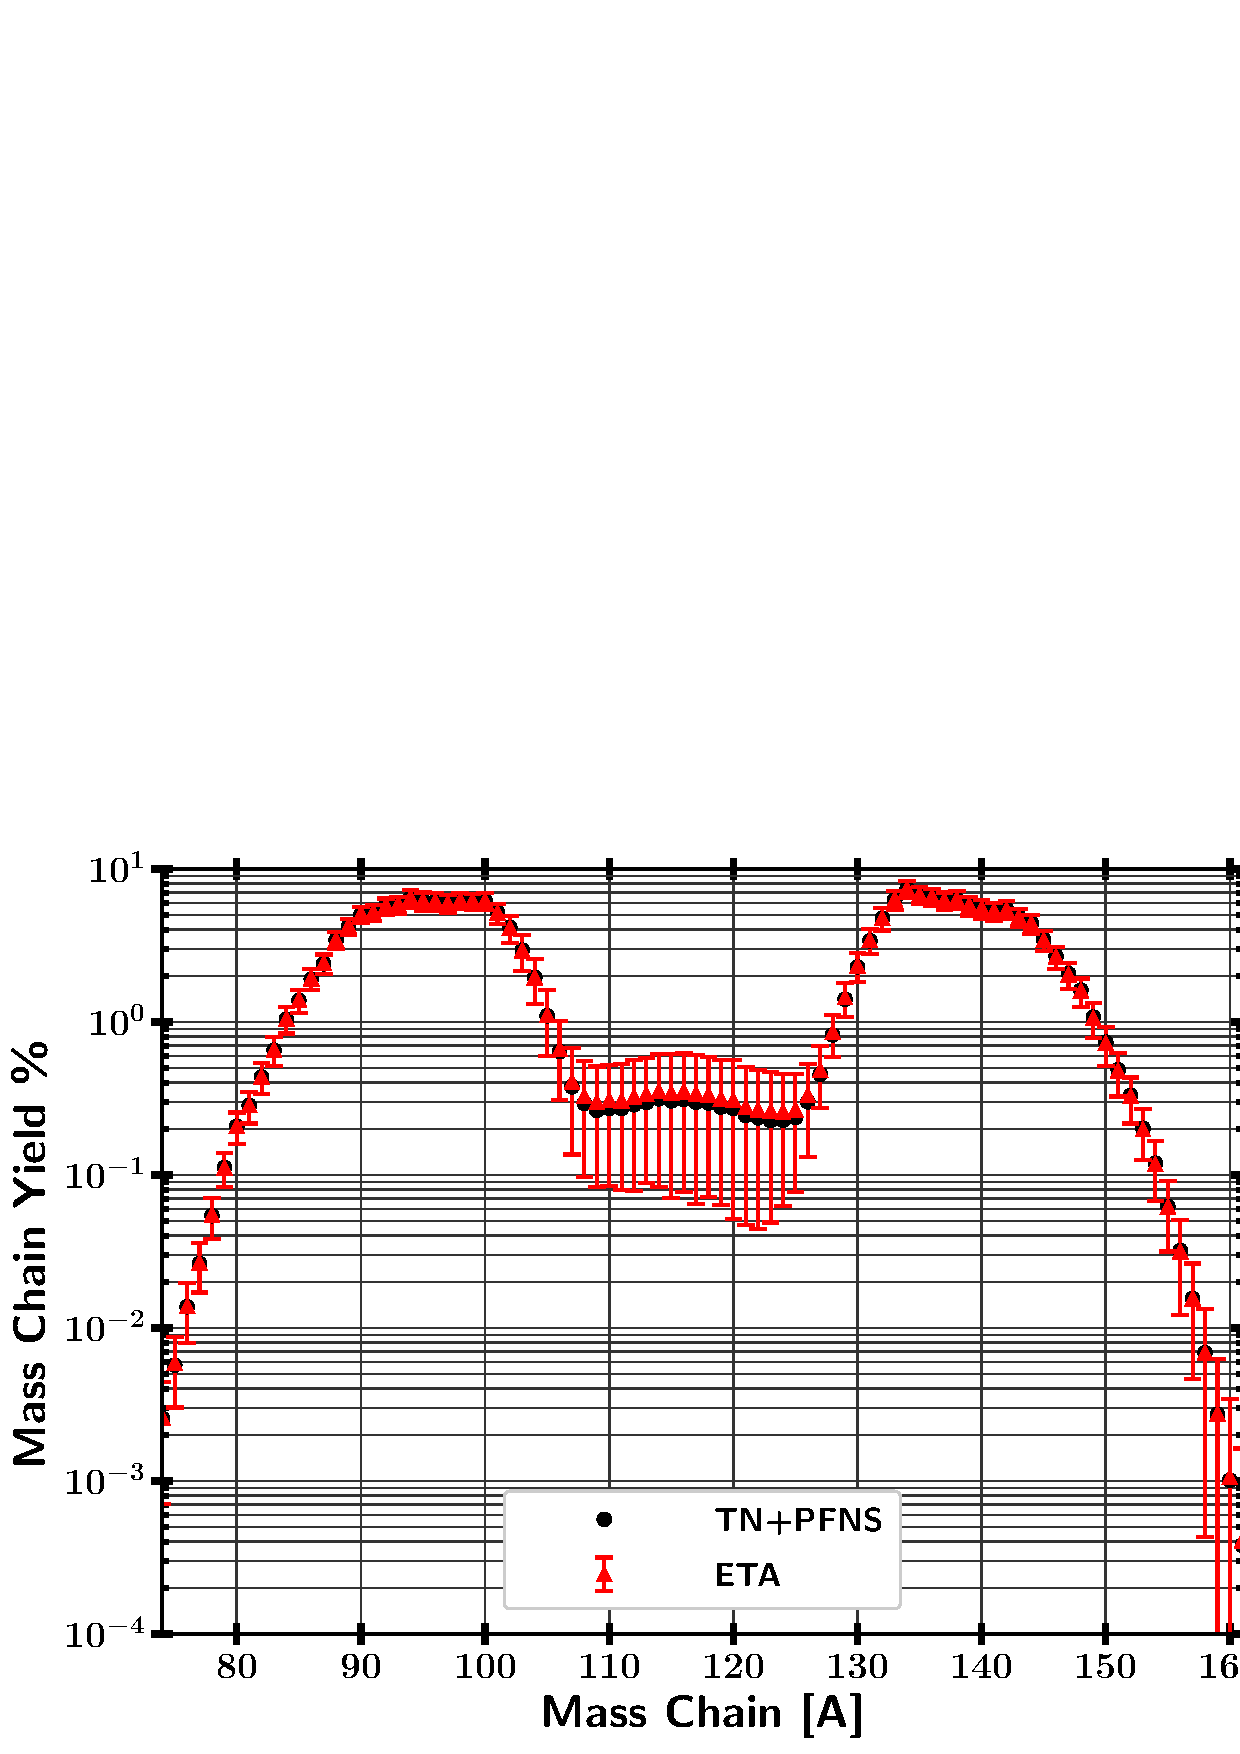
\includegraphics[width=13cm]{Figures/Chapter4/FPs/ETA_vs_TNPFNS_FPs.png}
	\caption{TN+PFNS versus ETA fission product mass chain distributions calculated with GEF values.}
	\label{fig:fp2}
\end{figure}

\ The mass chain residual yields comparing ETA to the objective spectrum are shown in Figure \ref{fig:fp3}. 
There are a few areas of disagreement between the mean value of ETA and the TN+PFNS. 
The symmetric valley fission products are systematically larger due to the increased high energy flux produced by ETA as highlighted in Table \ref{table:frac_flux}. 
Accordingly, the is an increase in yield for asymmetric fission products mass chains.
However, neither are substantial compared to the error. 

\begin{figure}[!htbp]
	\centering
	\includegraphics[width=13cm]{Figures/Chapter4/FPs/Residuals_Obj_minus_ETA.png}
	\caption{Residual mass chain yields of ETA compared to TN+PFNS from GEF values.}
	\label{fig:fp3}
\end{figure}

\subsection{Nagy Fits}

\ The experimental data as a function of incident neutron energy is applied to the ETA fluence with Nagy fits. 
The Nagy fit values represent the cumulative fission product yield for the individual isotope. 
The experimental parameters for the exponential slope of the fit and yield at thermal fission are shown in Figures \ref{fig:nagy1} and \ref{fig:nagy2}. 

\begin{figure}[!htbp]
	\centering
	\includegraphics[width=13cm]{Figures/Chapter4/FPs/U_Fis_FitParam.png}
	\caption{Nagy fit experimental data exponential slope values as a function of selected isotopes atomic mass.}
	\label{fig:nagy1}
\end{figure}

\begin{figure}[!htbp]
	\centering
	\includegraphics[width=13cm]{Figures/Chapter4/FPs/U_Fis_FitParam_Y0_lin.png}
	\caption{Nagy fit experimental data thermal fission yields as a function of selected isotopes atomic mass.}
	\label{fig:nagy2}
\end{figure}

The results of the fitting parameters are consistent with expectations. 
The yield at thermal fission fitting value is very similar to the mass chain distributions outlined in Figure \ref{fig:U235Cumulative}. 
The exponential slope of the cumulative yield as a function of energy is small for wing and peak mass chains which generally decrease with increasing incident neutron energy. 
The cumulative yields above mass chain 145 also slightly increase with neutron energy. 
The symmetric valley fission product yield increases much more substantially as shown by the large values of the exponential slope near the 110 mass number. 

The resultant fission product yields are compared between ETA and the objective TN+PFNS in Table \ref{table:fps3} along with the relative activities compared to $\mathrm{^{95}}$Zr. 
The isotope $\mathrm{^{95}}$Zr has a longer half-life and a strong gamma-ray to use as a baseline for comparison to the other fission products. 

\begin{table}[htb!]
	\centering
	\caption[ETA and TN+PFNS produced Nagy fit cumulative fission product yield from experimental data.]{ETA and TN+PFNS produced Nagy fit cumulative fission product yield from experimental data. The fission product activities are compared to the longer-lived $\mathbf{^{95}}$Zr}.
	\label{table:fps3}
	
	\setlength\extrarowheight{2.5pt}
	\resizebox{\textwidth}{!}{%
		\begin{tabular}{|c|c|c|c|c|}
\hline
\multirow{2}{*}{\begin{tabular}[c]{@{}c@{}}\textbf{Fission} \\ \textbf{Product} \end{tabular}} & \multicolumn{2}{c|}{\textbf{Fission Product Yield {[}\%{]}}} & \multicolumn{2}{c|}{\textbf{Relative Activity to $\mathrm{^{95}Zr}$}} \\ \cline{2-5} 
& \textbf{ETA} & \textbf{TN+PFNS} & \textbf{ETA} & \textbf{TN+PFNS} \\ \hline
$\mathrm{^{91}Sr}$ & 5.34 $\pm$ 0.15 & 5.37 $\pm$ 0.08 & 141 $\pm$ 3.7\% & 141 $\pm$ 1.7\% \\ \hline
$\mathrm{^{92}Sr}$ & 5.38 $\pm$ 0.16 & 5.41 $\pm$ 0.10 & 516 $\pm$ 4.0\% & 517 $\pm$ 2.1\% \\ \hline
$\mathrm{^{95}Zr}$ & 6.03 $\pm$ 0.15 & 6.05 $\pm$ 0.06 & 1 $\pm$ 3.6\% & 1 $\pm$ 1.3\% \\ \hline
$\mathrm{^{97}Zr}$ & 5.71 $\pm$ 0.16 & 5.74 $\pm$ 0.08 & 87.0 $\pm$ 3.7\% & 87.0 $\pm$ 1.7\% \\ \hline
$\mathrm{^{99}Mo}$ & 5.62 $\pm$ 0.16 & 5.65 $\pm$ 0.08 & 21.7 $\pm$ 3.8\% & 21.7 $\pm$ 1.7\% \\ \hline
$\mathrm{^{103}Ru}$ & 3.20 $\pm$ 0.09 & 3.21 $\pm$ 0.05 & 0.867 $\pm$ 3.8\% & 0.864 $\pm$ 1.8\% \\ \hline
$\mathrm{^{105}Ru}$ & 1.41 $\pm$ 0.05 & 1.39 $\pm$ 0.04 & 81.3 $\pm$ 4.6\% & 79.7 $\pm$ 3.0\% \\ \hline
$\mathrm{^{109}Pd}$ & 0.32 $\pm$ 0.02 & 0.29 $\pm$ 0.02 & 6.01 $\pm$ 6.3\% & 5.31 $\pm$ 5.6\% \\  \hline
$\mathrm{^{111}Ag}$ & 0.28 $\pm$ 0.01 & 0.25 $\pm$ 0.01 & 0.399 $\pm$ 4.8\% & 0.350 $\pm$ 3.7\% \\ \hline
$\mathrm{^{112}Pd}$ & 0.27 $\pm$ 0.01 & 0.23 $\pm$ 0.01 & 3.22 $\pm$ 5.9\% & 2.82 $\pm$ 5.4\% \\ \hline
$\mathrm{^{113}Ag}$ & 0.20 $\pm$ 0.01 & 0.18 $\pm$ 0.01 & 9.50 $\pm$ 7.0\% & 8.30 $\pm$ 6.5\% \\ \hline
$\mathrm{^{115g}Cd}$ & 0.28 $\pm$ 0.01 & 0.25 $\pm$ 0.01 & 1.36 $\pm$ 5.6\% & 1.18 $\pm$ 4.9\% \\ \hline
$\mathrm{^{132}Te}$ & 4.32 $\pm$ 0.13 & 4.33 $\pm$ 0.07 & 14.3 $\pm$ 3.9\% & 14.3 $\pm$ 1.9\% \\ \hline
$\mathrm{^{140}Ba}$ & 5.56 $\pm$ 0.15 & 5.60 $\pm$ 0.07 & 4.63 $\pm$ 3.7\% & 4.65 $\pm$ 1.6\% \\ \hline
$\mathrm{^{141}Ce}$ & 5.46 $\pm$ 0.17 & 5.49 $\pm$ 0.10 & 1.78 $\pm$ 4.0\% & 1.79 $\pm$ 2.1\% \\ \hline
$\mathrm{^{143}Ce}$ & 5.06 $\pm$ 0.15 & 5.11 $\pm$ 0.09 & 39.1 $\pm$ 3.9\% & 39.3 $\pm$ 1.9\% \\  \hline
$\mathrm{^{144}Ce}$ & 4.69 $\pm$ 0.16 & 4.75 $\pm$ 0.11 & 0.175 $\pm$ 4.2\% & 0.176 $\pm$ 2.5\% \\ \hline
$\mathrm{^{147}Nd}$ & 2.08 $\pm$ 0.06 & 2.10 $\pm$ 0.03 & 2.01 $\pm$ 3.8\% & 2.02 $\pm$ 1.7\% \\ \hline
$\mathrm{^{149}Pm}$ & 1.01 $\pm$ 0.04 & 1.01 $\pm$ 0.03 & 4.83 $\pm$ 4.9\% & 4.84 $\pm$ 3.3\% \\ \hline
$\mathrm{^{151}Pm}$ & 0.47 $\pm$ 0.02 & 0.46 $\pm$ 0.02 & 1361 $\pm$ 5.5\% & 1341 $\pm$ 4.3\% \\ \hline
$\mathrm{^{153}Sm}$ & 0.18 $\pm$ 0.01 & 0.18 $\pm$ 0.01 & 0.982 $\pm$ 6.6\% & 0.969 $\pm$ 5.5\% \\ \hline
$\mathrm{^{156}Eu}$ & 0.028 $\pm$ 0.001 & 0.027 $\pm$ 0.001 & 0.020 $\pm$ 5.4\% & 0.019 $\pm$ 4.3\% \\ \hline
$\mathrm{^{161}Tb}$ & 0.0013 $\pm$ 0.00006 & 0.0011 $\pm$ 0.00004 & 0.0020 $\pm$ 5.5\% & 0.0017 $\pm$ 4.2\% \\ \hline
		\end{tabular}%
	}
\end{table}

\ The cumulative fission product yields in Table \ref{table:fps3} are mostly the precursor to the stable state. 
In the case where there are additional steps in the decay chain before the stable state, the independent yield of daughter isotopes often have negligible yields.
Therefore, all of the decay feeding passes through these cumulative fission product isotopes with the exception of $\mathrm{^{132}}$Te. 
$\mathrm{^{132}}$Te is in competition with the daughter isotope $\mathrm{^{132}}$I. 
Therefore, the experimental yields, with the exception provided, enable lower uncertainty approximations of the mass chain yields than GEF where experimental data exists. 
Figure \ref{fig:fp4} displays the ETA results with Nagy fit data in their given mass chains, which substantially improves the picture of predicting fission product yields. 
In particular, these isotopes serve as excellent verification data points for the ETA experiment in confirming the ETA fission products. 

\begin{figure}[!htbp]
	\centering
	\vfill
	\subfigure[Logarithmic energy scale]{\includegraphics[width=13cm]{Chapter4/FPs/GEF_ENDF_Nagy.png}}
	\vfill
	\subfigure[Linear energy scale]{\includegraphics[width=13cm]{Chapter4/FPs/GEF_ENDF_Nagy_lin.png}}
	\vfill
	\caption{Experimental predictions of ETA mass chain yields utilizing GEF and Nagy fit data where selected experimental measurements exist in literature.}
	\label{fig:fp4}
\end{figure}

In a real world scenario, these fallout particles may be collected on the ground or air as with the CTBT monitoring. 
The Department of Defense Fallout Prediction System, DELFIC, can model the fallout distribution on the ground following a nuclear event with the Fallout Planning Tool user interface \cite{DELFIC, Jodoin2011}. 
A 10 KT fission weapon at ground level was modeled using weather data from 16 August 2017 at Wright-Patterson Air Force Base, OH. 
The ground dispersal in effective fissions per meter square from the 140 mass chain is shown in Figure \ref{fig:delfic}.
The 140 mass chain was chosen because the yield does not change drastically with the fissioning system. 
The modeled ETA results produced an equivalent number of fissions as in 0.1 m$^{2}$ of the lowest contour band. 
As the number of fissions are increased, the quality of the sample is more useful. 
Nevertheless, the modeled ETA performance has promising capabilities to create spectrally accurate fission product debris. 

\begin{figure}[!htbp]
	\centering
	\includegraphics[width=13cm]{Figures/Chapter5/FP_m2.png}
	\caption{DELFIC calculated fission product equivalent fissions on the ground per unit area from mass chain 140.}
	\label{fig:delfic}
\end{figure}

